\section{Measuring \textit{in vivo} turnover rates with smPReSS}

Dynamic remodeling of the embryonic cell surface is essential for the control of cell polarity, division, shape change and movement during early development. This remodeling involves the local movement and exchange of proteins at the interface between the plasma membrane and the actin-rich cell cortex. Quantifying these processes in vivo remains a challenge. One promising approach is single-molecule imaging combined with SPT, which can yield quantitative measurements of local mobilities, binding states and exchange kinetics that are inaccessible with ensemble measurements\cite{doi:10.1021/ac9024889}. Combining these approaches with genetic tools in a classical model organism could be a powerful way to investigate subcellular dynamics in embryonic cells.

One key impediment to performing such experiments has been the lack of simple and reliable methods for tunable and noninvasive labeling of target molecules. Optimal labeling densities are different for each target and must balance the need for high-density sampling of molecular behavior against practical requirements for accurate and unbiased single-molecule detection and tracking. Toward the goal of measuring molecular remodeling and actomyosin dynamics, we developed a simple, versatile and minimally invasive method\cite{nmeth} for single-molecule imaging at the cell surface in C. elegans embryos of transgenic strains expressing GFP-tagged actin proteins. In particular, we showed how these data could be used to extract quantitative information about surface density and turnover.


\subsection{smPReSS measurement technique}



We sought to exploit the intrinsic exchange dynamics of surface-associated proteins to create a self-renewing pool of GFP-tagged single molecules at the cell surface that could be followed over time to measure mobility and turnover. To establish a kinetic basis for this approach, we consider a GFP-tagged protein that exchanges dynamically between the bulk cytoplasm and a region of the cell surface, which is observed by near-TIRF microscopy (Fig. \ref{fig:smpress}a). The number of molecules N(t) within this region over time is governed by

\begin{equation}
\frac{dN}{dt} = k_{app}-(k_{off}+k_{ph})N
\end{equation}

where $k_{app}$ is an observable appearance rate that depends on the cytoplasmic concentration of GFP-tagged protein ($k_{app} = k_{on} \times Y$, where $Y$ is the cytoplasmic concentration) and the nature of the binding process. $k_{off}$ and $k_{ph}$ are pseudo-first-order rate constants such that $k_{off} \times N$ is the rate (in molecules per second) at which particles disappear owing to unbinding or disassembly, and $k_{ph} \times N$ is the rate (in molecules per second) at which they disappear owing to irreversible photobleaching (Fig. \ref{fig:smpress}a). Prior to illumination, $k_{ph} = 0$ and the steady state density is $N_{ss} \approx k_{app}/k_{off}$. During illumination, $k_{ph}$ becomes nonzero; if the cytoplasmic pool were infinite, the system would approach a new steady-state density given by $N_{ssobs} = k_{app}/(k_{off} + k_{ph})$, which is a fixed fraction $f = k_{off}/(k_{off} + k_{ph})$ of the initial unobserved value (Fig. \ref{fig:smpress}b). In practice, irreversible photobleaching will gradually deplete a finite cytoplasmic pool. A variant of the kinetic model that accounts for this depletion predicts a biphasic response to the onset of illumination: a fast relaxation toward $N_{ssobs}$ followed by a slower decay toward 0, at a rate that depends on the photobleaching rate and the size of the cytoplasmic pool (Fig. \ref{fig:smpress}b). For a given target molecule, $k_{off}$ is fixed. However, $k_{ph}$ depends on imaging conditions (i.e., the intensity and duty ratio of the laser illumination), and $k_{app}$ can be adjusted by tuning the initial size of the GFP-tagged pool. Thus, co-tuning these factors should make it possible to target a desired density $N_{ssobs}$ at quasi-steady state for a range of imaging conditions.

\begin{figure}[H]
	\centering
	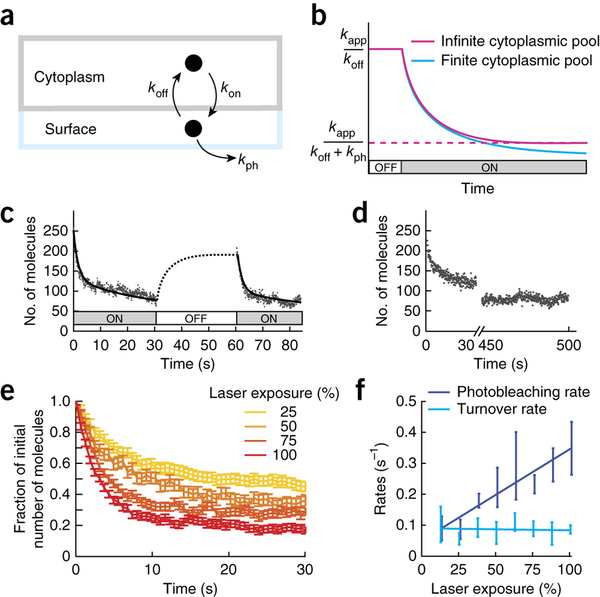
\includegraphics[width=0.8\hsize]{nmeth/nmeth.jpg}
	\caption{\label{fig:smpress} smPReSS measurement technique.  \textbf{a)}  The basic kinetic principle: during imaging, the level of surface-associated proteins is set by a dynamic balance of appearance (binding or assembly) at an observable rate $k_{app}$, disappearance (unbinding or disassembly) at a per-molecule rate $k_{off}$, and photobleaching at a per-molecule rate $k_{ph}$.  \textbf{b)} Predicted response of an initially unobserved cell at steady state to a step change in illumination. For an infinite cytoplasmic pool, the surface density relaxes to a new illuminated steady state. For a finite cytoplasmic pool, fast relaxation is accompanied by a slower decay caused by irreversible photobleaching. \textbf{c)} Fast relaxation to a quasi-stable density during illumination is rapidly reversed when the laser is turned off. \textbf{d)}  Biphasic response for GFP::actin under illumination conditions that allow accurate single-molecule detection and tracking. Time from $t$ = 30-450 s is discontinuous. \textbf{e)} Surface density of GFP::actin vs. time at various laser exposures, shown as a fraction of the initial unobserved density. Error bars, s.e.m. ($n$ = 7, 9, 6, 7 embryos for laser exposures from low to high). textbf{f)} Estimates of per-molecule turnover ($k_{off}$) and photobleaching ($k_{ph}$) rates as a function of laser exposure. Error bars, s.d. (n = 12, 7, 8, 9, 7, 6, 7, 7 embryos, low to high laser exposure). Solid lines show a linear regression against the data. 100\% laser power $\approx 1.6 \mu W/\mu m^2$.} 
	
\end{figure}

To test this approach, we chose a representative strain that expressed GFP::actin. Actin monomers exchange dynamically with the cell surface through local filament assembly and disassembly, and on the basis of previous work, we expected GFP::F-actin to be relatively immobile at the cell surface and to turn over in a few tens of seconds. In contrast, fast-diffusing monomers of GFP::G-actin should produce highly blurred images and thus escape detection under our imaging conditions6. Focusing again on the polarity maintenance phase, we reduced densities to single-molecule levels, allowed the system to equilibrate unobserved and then recorded data for a range of laser intensities and exposure times (Fig. \ref{fig:smpress}c–e). We observed the predicted biphasic response to a step change in illumination: a rapid initial decrease in the number of molecules to a quasi-stable value followed by slower decay (Fig. \ref{fig:smpress}c,d). Notably, the initial decrease was reversed with equally rapid kinetics when the laser was turned off (Fig. \ref{fig:smpress}c), a result confirming that the quasi-steady state is set by a dynamic balance of exchange and photobleaching. We could therefore obtain robust estimates for effective dissociation and photobleaching rate constants $k_{off}$ and $k_{ph}$ by fitting the predicted biphasic kinetics to the change in single-molecule density over time; for each strain, we optimized fitting conditions by adjusting laser exposure. As expected, estimates of $k_{ph}$ varied linearly with laser exposure, whereas estimates of $k_{off}$ remained fixed over a range of exposures (Fig. \ref{fig:smpress}f). Our estimate of $k_{off}$ for actin::GFP of $koff = 0.1 ± 0.07 s^{−1}$ demonstrates that actin filaments astonishingly short-lived, with a typical lifetime of only approximately 10s.



\subsection{Measurements of turnover rate in dividing \textit{C. elegans} cortex}



We measured spatiotemporal modulation of actin assembly and disassembly during the first cell division in the C. elegans embryo (Fig. \ref{fig:meas_div}a). Both actin assembly and disassembly are thought to be modulated during cytokinesis, but their relative contributions to actin filament accumulation are not well understood. We performed these experiments in embryos depleted of nonmuscle myosin II to remove the confounding effects of surface deformations and flow and to remove myosin-dependent effects on turnover. We verified strong depletion of myosin II by the complete failure of cytokinesis and a complete absence of local surface deformation and cortical flow during early anaphase. In the case of GFP::actin, the turnover rates measured by smPReSS ($k_{off} \approx 0.1 s^{−1}$) were similar to the photobleaching rates ($k_{ph} \approx 0.1 s^{−1}$) required for accurate particle tracking and agreed well with estimates of $k_{off}$ from particle tracking (Fig. \ref{fig:meas_div}b), suggesting that in this case, we could use SPT to measure spatiotemporal variations in turnover, with the smPReSS measurements of $k_{ph}$ used to correct for photobleaching. We measured roughly uniform values for $k_{app}$ and $k_{off}$ along the anterior-posterior axis during maintenance phase (Fig. \ref{fig:meas_div}c–e), a result consistent with a lack of cortical asymmetry at this stage in myosin-depleted embryos. During the transition into anaphase, when the contractile ring normally assembles, we observed a net increase in actin density at the equator as anticipated, and we also observed a net decrease at the poles (Fig. \ref{fig:meas_div}a,c). Surprisingly, these changes involved strong modulation of both filament assembly and disassembly (Fig. \ref{fig:meas_div}d,e). The equatorial increase was associated with a small increase in assembly rate and a larger decrease in turnover, whereas the polar decrease in density was associated with both a decrease in assembly and an increase in turnover. Thus, our ability to simultaneously resolve assembly, disassembly and density revealed an unappreciated dimension to the control of cortical microfilaments during cell division.

\begin{figure}[H]
	\centering
	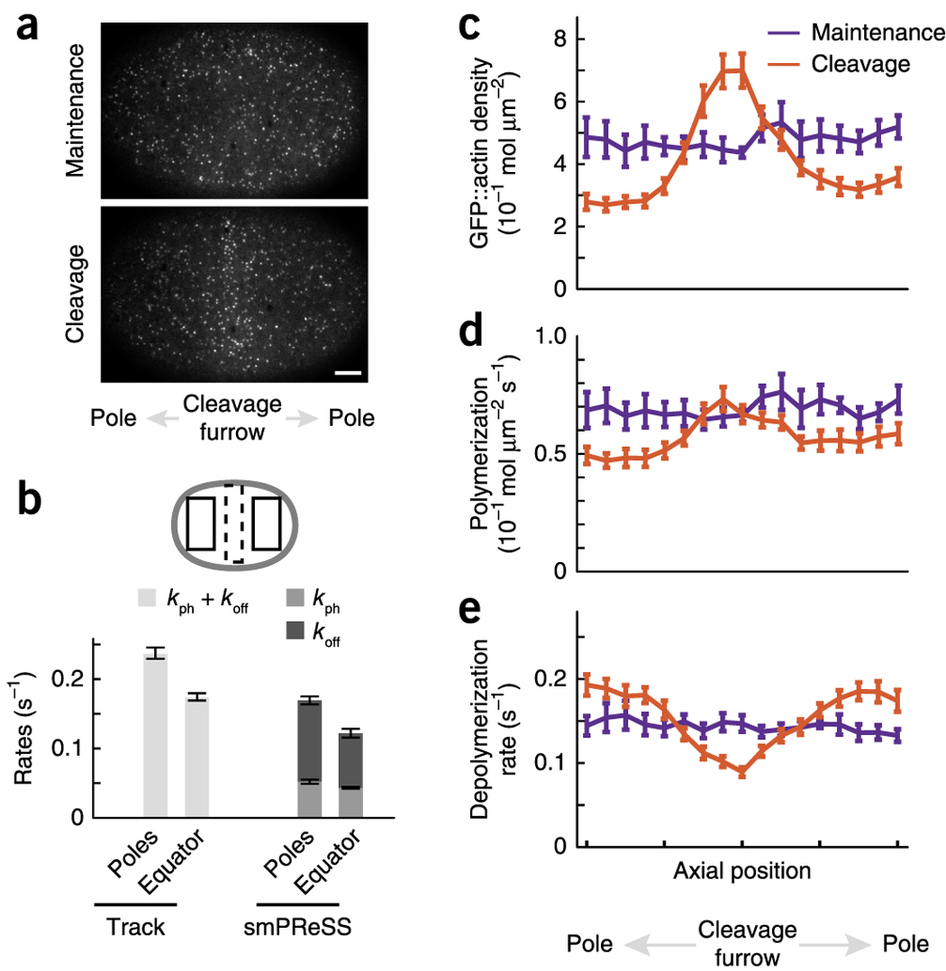
\includegraphics[width=0.8\hsize]{nmeth/nmethF4.jpg}
	\caption{\label{fig:meas_div}Measurement of cortical actin lifetimes.  \textbf{a)} Near-TIRF micrographs of GFP::actin during the polarity maintenance phase (top) and cleavage (bottom). \textbf{b)} Measurements of the indicated turnover rates at the equator and poles during anaphase using tracking (left) or smPReSS (right). Schematic indicates the equatorial (dashed box) and polar (solid boxes) regions in which the measurements were made. For tracking, the sum of koff and kph is displayed; for smPReSS, the values for $k_{ph}$ and $k_{off}$ are stacked. \textbf{c-e)} Spatial variation in actin density and turnover kinetics during maintenance phase and cleavage measured by tracking and binned along the antero-posterior axis. \textbf{c)} Cortical density. \textbf{d)} Polymerization rate. \textbf{e)} Depolymerization rate (instantaneous disappearance rate minus estimated photobleaching rate). In b-e, error bars indicate cell-to-cell s.e.m. (n = 7 embryos, maintenance, and n = 16 embryos, cleavage). Scale bar, $5 \mu m$.} 
	
\end{figure}